%=================================================================
% sOFIa - LabDST - Corte 1 draft
% Version: v0.2 (2026-09-21)
% Scope: Introduction + Related Work + Materials and Methods
%=================================================================
\documentclass[lettersize,journal]{IEEEtran}

\usepackage{amsmath,amsfonts}
\usepackage{array}
\usepackage{graphicx}
\usepackage{cite}
\usepackage{url}
\usepackage{textcomp}
\usepackage{float}
\usepackage{placeins}
\usepackage{algorithm}
\usepackage{algpseudocode}
\usepackage[caption=false,font=normalsize,labelfont=sf,textfont=sf]{subfig}
\usepackage{tabularx}
\usepackage{balance}

\hyphenation{op-tical net-works semi-conduc-tor}
\def\BibTeX{{\rm B\kern-.05em{\sc i\kern-.025em b}\kern-.08em
        T\kern-.1667em\lower.7ex\hbox{E}\kern-.125emX}}

\begin{document}

\title{Technical Architecture and Kinematic Modeling of sOFIa, an Interactive Robotic Artistic System}

\author{Juan Mauricio Serna G\'omez, Alejandro Rodr\'iguez Veloquio, Francisco Uriel Padilla Pedroza, Diego Rosales Rojas, Jorge A. Lizarraga, Graciela Baca, Luis Enrique Gonz\'alez-Jim\'enez and Luis F. Luque-Vega%
\thanks{The authors are with ITESO, Tlaquepaque 45604, Jalisco, Mexico.}}

\markboth{LabDST -- sOFIa -- Corte 1 -- v0.2}%
{Serna G\'omez \MakeLowercase{\textit{et al.}}: Preliminary Architecture and Kinematic Modeling of sOFIa}

\maketitle

\begin{abstract}
sOFIa is an interactive robotic artistic system able to establish visual comunication between people and a mechatronic array (that is also modular). The platform combines a camera and a PC-based perception interface with an array of actuated hexagonal units. This work documents the Discover and Learn stages of the project by characterizing the reference system, formalizing its computational requirements, defining a preliminary perception-to-actuation architecture, and establishing the kinematic model used by the actuated modules. The implemented vision baseline uses MediaPipe hand landmarks with OpenCV and NumPy to recognize five hand-based interaction gestures, including three dynamic gestures, while optional body-pose association supports multi-user operation. Temporal landmark smoothing, output-rate limiting, a 16-module mapping stage, and a communication interface to the master ESP32 are incorporated as part of the preliminary software architecture. For the mechatronic side, a two-degree-of-freedom rotational model is expressed through sequential rotations and an inverse-kinematics mapping from a target direction to the joint variables. A MATLAB microtest implements a 16-unit honeycomb array following a moving three-dimensional point under explicit joint limits and singularity handling. The resulting methodology provides a traceable baseline for subsequent implementation, integration, and experimental validation of the complete gesture-reaction loop.
\end{abstract}

\begin{IEEEkeywords}
human--robot interaction, hand gesture recognition, human pose estimation, inverse kinematics, modular robotics, computer vision, robotic artistic system
\end{IEEEkeywords}

%=================================================================
\section{Introduction}
\label{sec:introduction}

\IEEEPARstart{s}{OFIa} is a robotic artistic interactive system based on intelligent vision. The reference system combines a mechatronic structure formed by actuated hexagonal panels, a PC, and a camera. Its intended interaction is visual: people inside the camera FOV produce body postures, the computational subsystem interprets those postures, and the mechatronic subsystem reacts through coordinated motion.

The technical challenge is not limited to pose estimation or to actuator control alone. The complete interaction loop must detect five postures in one or more persons, map those detections to mechanical reactions, exchange commands wirelessly between the PC and the master ESP32, provide an operator interface for visualization and debugging, and support performance evaluation of the integrated system \cite{labdst2026sc}. These requirements couple computer vision, communication, embedded control, and the kinematics of the actuated surface.

A useful formulation of the project question is: \emph{how can a camera-based multi-person interaction pipeline be integrated with a modular two-degree-of-freedom kinetic array so that hand-based postures and motions can be translated into bounded and reproducible mechanical reactions?} At the current Discover--Learn stage, the objective is to characterize the reference system, identify the technical decisions that constrain the solution, define a preliminary architecture and risk model, and establish a reproducible kinematic microtest before full hardware/software integration.

The main contribution of this "Corte 1" manuscript is consequently a traceable technical baseline rather than a final validated prototype. It connects the project requirements with a perception-framework selection rationale, a preliminary bill of materials (BOM), the mathematical orientation model of one sOFIa unit, and a simulation protocol for the 16-unit array. These elements define what must be implemented and measured during the subsequent Apply and Build \& Validate stages.

\subsection{Related Work}
\label{sec:related}

Real-time human-pose estimation provides the perception layer required by sOFIa. OpenPose introduced a bottom-up multi-person approach based on Part Affinity Fields, associating detected body parts with individual people while maintaining real-time operation independent of the number of people in the scene \cite{cao2017openpose}. This directly addresses the need to extract body keypoints from multiple users, although it does not by itself define the application-specific posture vocabulary or the downstream mechatronic response.

MediaPipe was proposed as a framework for constructing perception pipelines with explicit attention to cross-platform deployment, resource consumption, and iterative prototyping \cite{lugaresi2019mediapipe}. The current sOFIa vision prototype adopts the MediaPipe ecosystem for hand-landmark extraction, while an optional body-pose stage is used to associate detected hands with people in multi-user scenes. BlazePose remains relevant as a lightweight real-time body-pose reference within the same ecosystem \cite{bazarevsky2020blazepose}.

The project definition also identifies YOLO-based pose estimation as a candidate and includes the Ultralytics package in the general software framework \cite{labdst2026sc}. YOLO11 provides pretrained pose/keypoint variants within the Ultralytics workflow \cite{jocher2024yolo11}; in the present Corte 1 implementation it is treated as a comparison alternative rather than as the selected gesture-recognition backend. Any future substitution of the vision backend must be justified through measurements under the project's camera, illumination, and multi-user conditions.

These approaches primarily solve the perception problem: they estimate people, hands, or skeletal keypoints from images or video. sOFIa additionally requires temporal gesture rules, smoothing against false positives, gesture-to-reaction semantics, a wireless command/acknowledgment layer, and bounded mechanical motion of the hexagonal array. The project gap is therefore an integration gap: adapting established landmark-estimation tools into a reproducible perception-to-actuation pipeline tailored to the sOFIa demonstrator.

%=================================================================
\section{Materials and Methods}
\label{sec:methods}

\subsection{Reference System and Functional Decomposition}
\label{sec:reference-system}

The reference architecture contains a PC/camera perception side and a distributed mechatronic side. According to the project specification, the PC acquires video, detects postures, presents the detection state through a GUI, and sends the corresponding reaction command wirelessly to a master ESP32. The mechatronic architecture distributes actuator commands through module electronics that include PCA9685 PWM drivers and an internal RS-485/Modbus-oriented bus between controller boards. The functional chain used in this work is
\begin{equation}
\begin{aligned}
\text{camera} &\rightarrow \text{landmarks} \rightarrow \text{gesture rule}\\
&\rightarrow \text{reaction command} \rightarrow \text{module motion}.
\end{aligned}
\label{eq:functional-chain}
\end{equation}

Table~\ref{tab:requirements} converts the project specification into requirements that can later be verified experimentally. No numerical acceptance thresholds are invented at this stage; quantities such as accuracy, response time, and frame rate are to be measured during validation.

\begin{table}[H]
\centering
\caption{Preliminary functional and validation requirements derived from the sOFIa technical specification.}
\label{tab:requirements}
\scriptsize
\setlength{\tabcolsep}{2.5pt}
\begin{tabularx}{\columnwidth}{p{0.55cm}p{3.55cm}X}
\hline
\textbf{ID} & \textbf{Requirement} & \textbf{Verification evidence planned} \\
\hline
FR1 & Detect five designed hand-based interaction gestures for people inside the camera field of view, while retaining a path for multi-user association. & Live annotated video, per-gesture hit rate, and confusion/error records. \\
FR2 & Include at least three dynamic gestures whose recognition depends on more than one captured image. & Temporal rule traces and test sequences. \\
FR3 & Reduce spurious gesture detections caused by landmark noise and abrupt output changes. & Documented smoothing/debounce rule and false-positive comparison. \\
FR4 & Exchange gesture/reaction commands wirelessly between the PC and the master ESP32. & Message format, acknowledgments, error codes, and communication test. \\
FR5 & Provide a GUI for live video, detection state, execution control, and integration debugging. & Functional interface demonstration without blocking the processing thread. \\
FR6 & Characterize integrated detection performance. & Hit rate, response time, average FPS, and tests with different users and illumination conditions. \\
\hline
\end{tabularx}
\end{table}

\subsection{Vision Framework Selection}
\label{sec:pose-selection}

The project specification identifies YOLO, MediaPipe, OpenPose, and OpenCV DNN with a TensorFlow model as candidate vision approaches. For the current "Corte 1" prototype, the team selected a Python pipeline based on MediaPipe hand tracking, OpenCV, and NumPy. The selection is motivated by the ability to obtain 21 hand landmarks in real time without training a project-specific neural network, while OpenCV provides camera acquisition and visualization and NumPy supports the coordinate calculations used by the gesture logic. Table~\ref{tab:pose-comparison} retains the broader alternatives as part of the technical selection record rather than presenting them as implemented backends.

\begin{table}[H]
\centering
\caption{Qualitative comparison of vision alternatives considered for sOFIa and status in the Corte 1 prototype.}
\label{tab:pose-comparison}
\scriptsize
\setlength{\tabcolsep}{2.2pt}
\begin{tabularx}{\columnwidth}{p{1.35cm}p{2.15cm}p{2.15cm}X}
\hline
\textbf{Alternative} & \textbf{Relevant capability} & \textbf{Project consideration} & \textbf{Corte 1 status} \\
\hline
MediaPipe + OpenCV & Landmark-oriented perception pipeline suitable for real-time interaction \cite{lugaresi2019mediapipe}. & The team's implementation uses hand landmarks for the gesture vocabulary and can optionally associate hands with detected body poses. & \textbf{Selected and implemented baseline}. \\
OpenPose & Real-time multi-person 2-D pose with Part Affinity Fields \cite{cao2017openpose}. & Strong direct fit to multi-person body-keypoint extraction; integration and computational cost would need evaluation on the target PC. & Literature / comparison alternative. \\
YOLO11-pose & Unified Ultralytics pose/keypoint workflow \cite{jocher2024yolo11}. & Present in the general project framework, but not used as the current hand-gesture backend. & Comparison alternative. \\
OpenCV DNN + TensorFlow & Model-dependent inference path within the OpenCV ecosystem. & Flexible, but behavior and resource use depend on the selected network. & Fallback / comparison alternative. \\
\hline
\end{tabularx}
\end{table}

The prototype is implemented in Python with MediaPipe, OpenCV, and NumPy. Exact package and interpreter versions will be pinned in the project repository to preserve reproducibility.

\subsection{Gesture Vocabulary and Mechanical Reactions}
\label{sec:gesture-vocabulary}

The five interactions defined for the vision module are hand-based gestures. Three are dynamic, and two are static configurations with a one-second temporal hold condition. Table~\ref{tab:gestures} records the gesture semantics and the intended reaction of the kinetic array. These mappings are design specifications for the interaction loop; their recognition accuracy and mechanical execution will be quantified during later validation.

\begin{table}[H]
\centering
\caption{Five vision gestures and intended sOFIa reactions defined for the interaction prototype.}
\label{tab:gestures}
\scriptsize
\setlength{\tabcolsep}{2.5pt}
\begin{tabularx}{\columnwidth}{p{2.0cm}p{3.0cm}X}
\hline
\textbf{Gesture} & \textbf{Detection concept} & \textbf{Intended mechanical reaction} \\
\hline
Open-hand vertical displacement & Track an open hand moving upward or downward across successive frames. & Follow the user's hand in the vertical direction. \\
Open-hand horizontal displacement & Track an open hand moving left or right across successive frames. & Move from left to right, or in the corresponding horizontal direction, until the action stops. \\
Pulse: open--closed--open & Detect the temporal sequence of opening, closing, and reopening the hand. & Produce a pulse-like motion intended to simulate a heartbeat. \\
Sustained open palm & Keep the open-palm state stable for approximately 1~s. & Move all panels vertically and then horizontally once. \\
Sustained closed fist & Keep the closed-fist state stable for approximately 1~s. & Open the outer panels while closing the inner panels for approximately 3~s. \\
\hline
\end{tabularx}
\end{table}

\subsection{Real-Time Vision and Interaction Pipeline}
\label{sec:vision-pipeline}

The implemented software is organized as a camera-to-actuation pipeline,
\begin{equation}
\begin{aligned}
\text{camera} &\rightarrow \text{MediaPipe landmarks} \rightarrow \text{smoothing}\\
&\rightarrow \text{gesture engine} \rightarrow \text{16-module mapping}\\
&\rightarrow \text{master ESP32 interface}.
\end{aligned}
\label{eq:vision-chain}
\end{equation}
The camera runs in a dedicated capture thread whose policy is to retain the most recent frame and discard older buffered frames. This favors low interaction latency over exhaustive frame processing. MediaPipe inference is handled asynchronously by the tracker backend, while the main loop draws the overlays, evaluates gesture events, updates the module command matrix, and performs communication. The current front end is an OpenCV visualization/control window, being the development interface rather than the final GUI required in the later integration stage.

Hand detections are smoothed independently using a persistent landmark filter keyed to each observed hand. When optional body-pose tracking is enabled, detected hands are associated with body poses so that the software can maintain a person-related identity in multi-user scenes. This association supports the project requirement for several people without changing the hand-based definition of the five gestures.

A second stabilization stage acts on the 16-module command vector through a slew-rate limiter with a deadband. The purpose of this stage is different from landmark smoothing: the former limits abrupt actuator-command changes, while the latter attenuates measurement jitter before gesture classification. Gesture events can be sent individually to the master ESP32, and the full 16-element command matrix can be transmitted periodically at a configurable rate. The communication object also provides an initial handshake, acknowledgment checking for gesture messages, connection maintenance, and a safe stop operation when the application closes.

\subsection{Vision Microtest and Data-Acquisition Plan}
\label{sec:vision-metrics}

The current application already exposes the variables required for the first vision microtests. When metric logging is enabled, each processed iteration can record timestamp $t_k$, mean frame rate $FPS_k$, number of detected hands $N_{h,k}$, emitted gesture  $g_k$, gesture confidence $c_k$, and loop latency $\tau_k$. These fields define the initial acquisition format:
\begin{equation}
\mathcal{D}_k=\{t_k,\; FPS_k,\; N_{h,k},\; g_k,\; c_k,\; \tau_k\},
\label{eq:vision-dataset}
\end{equation}
For "Corte 1", Eq.~(\ref{eq:vision-dataset}) defines how performance evidence will be collected; no accuracy, FPS, or latency result is claimed until controlled trials have been executed.

The planned validation will exercise each of the five gestures with different users and illumination conditions, including scenes with more than one person when pose association is enabled. At minimum, the later analysis will report gesture hit rate, false activations, response time, and average FPS, matching the performance categories defined in the project specification \cite{labdst2026sc}. This separation between an implemented acquisition mechanism and future measured results keeps the present section methodological rather than prematurely reporting unverified performance.

\subsection{Preliminary Bill of Materials and Key Components}
\label{sec:bom}

The demonstrator BOM supplied as a starting point contains two PCA9685 PWM drivers, one ESP32-C3 Super Mini board, 32 MG90S servomotors, one RS-485/Modbus driver, a pair of JST-VH connectors, and the PCB/enclosure assembly.

\begin{table}[H]
	\caption{Preliminary Bill of Materials for the sOFIa Demonstrator}
	\label{tab:bom}
	\centering
	\footnotesize
	\setlength{\tabcolsep}{3pt}
	\renewcommand{\arraystretch}{1.15}
	\begin{tabular}{p{0.16\columnwidth} p{0.48\columnwidth} c p{0.18\columnwidth}}
		\hline
		\textbf{Component} & \textbf{Technical Description} & \textbf{Qty.} & \textbf{Manufacturer / Origin} \\
		\hline
		
		PCA9685 &
		16-channel, 12-bit PWM controller for servo actuation &
		2 &
		NXP \\
		
		ESP32-C3 Super Mini &
		Wi-Fi/BLE microcontroller used as master controller &
		1 &
		Espressif \\
		
		MG90S &
		Micro servo used for the two rotational DOF of each module &
		32 &
		YSIDO, China \\
		
		RS-485 driver &
		Differential communication interface for the distributed bus &
		1 &
		Stlxy, China \\
		
		JST-VH &
		Power/interconnection connectors, male and female &
		2 &
		China \\
		
		PCB + enclosure &
		Custom electronic integration and mechanical protection &
		1 &
		Local fabrication \\
		\hline
	\end{tabular}
\end{table}

\subsection{Kinematic Model of One sOFIa Unit}
\label{sec:kinematics}

Each hexagonal unit is modeled as a two-degree-of-freedom rotational mechanism actuated by two servomotors. Let $q_1$ denote the first rotation about the local $x$ axis and $q_2$ the second rotation about the displaced local $y$ axis. The orientation of the output platform is \cite{lizarraga2026kinematics}
\begin{equation}
\mathbf{R}_{1,2}=\mathbf{R}_x(q_1)\mathbf{R}_y(q_2).
\label{eq:R12}
\end{equation}
The order in Eq.~(\ref{eq:R12}) is physically significant because the second servo rotates about an axis already displaced by the first rotation \cite{lizarraga2026kinematics}.

For an output direction initially aligned with the local $+z$ axis, the corresponding unit vector after the two rotations is
\begin{equation}
\hat{\mathbf r}_{2,3}=
\begin{bmatrix}
\sin q_2\\
-\cos q_2\sin q_1\\
\cos q_1\cos q_2
\end{bmatrix}.
\label{eq:r23hat}
\end{equation}
Let $\mathbf p$ be the target point and $\mathbf r_{0,2}^{(i)}$ the origin of the output frame of module $i$. The desired pointing direction is
\begin{equation}
\hat{\mathbf r}_{2,p}^{(i)}=
\frac{\mathbf p-\mathbf r_{0,2}^{(i)}}{\left\|\mathbf p-\mathbf r_{0,2}^{(i)}\right\|}
=\begin{bmatrix}u_x & u_y & u_z\end{bmatrix}^{\!T}.
\label{eq:desired-direction}
\end{equation}
Equating Eqs.~(\ref{eq:r23hat}) and (\ref{eq:desired-direction}) gives the inverse-kinematics solution used in the project material \cite{lizarraga2026kinematics}:
\begin{align}
q_2 &= \arcsin(u_x), \label{eq:q2}\\
q_1 &= \operatorname{atan2}(-u_y,u_z). \label{eq:q1}
\end{align}

A singular configuration occurs when $u_x=\pm1$, which implies $\cos q_2=0$ and $u_y=u_z=0$; in that case $q_1$ is not determined by the pointing direction \cite{lizarraga2026kinematics}. For the simulation microtest, the adopted numerical rule is to retain the previous valid $q_1$ value (or $q_1=0$ at initialization) whenever $\sqrt{u_y^2+u_z^2}<10^{-9}$. After inverse kinematics, both joint variables are limited to the selected physical range:
\begin{equation}
q_j^{\mathrm{cmd}}=\operatorname{clip}\left(q_j,-45^{\circ},45^{\circ}\right),\quad j\in\{1,2\}.
\label{eq:clamp}
\end{equation}

\subsection{MATLAB Kinematic Microtest}
\label{sec:simulation}

A MATLAB microtest was prepared to exercise the inverse-kinematics mapping before hardware integration. The code defines 16 module origins in a centered honeycomb arrangement with a pitch of $0.12$~m. The fixed dimensions are $z_{1,2}=0.020$~m and $z_{2,3}=0.030$~m, and both joint variables are constrained to $\pm45^{\circ}$. The moving target follows
\begin{equation}
\mathbf p(t)=
\begin{bmatrix}
0.15\cos(0.3t)\\
0.15\sin(0.3t)\\
0.40
\end{bmatrix}\ \mathrm{m},
\label{eq:trajectory}
\end{equation}
for 25~s with a simulation step of 0.4~s. These values reproduce the uploaded simulation configuration.

Algorithm~\ref{alg:ik} summarizes the language-independent computation applied to each module. The corrected MATLAB source accompanying this draft uses the same rotation order as Eq.~(\ref{eq:R12}) for visualization.

\begin{algorithm}[H]
\caption{Inverse-kinematics update for one sOFIa unit}
\label{alg:ik}
\begin{algorithmic}[1]
\Require Module origin $\mathbf r_{0,2}$, target $\mathbf p$, joint limits $q_{j,\min},q_{j,\max}$
\Ensure Bounded commands $q_1^{\mathrm{cmd}},q_2^{\mathrm{cmd}}$
\State $\mathbf d\gets\mathbf p-\mathbf r_{0,2}$
\State $\mathbf u\gets\mathbf d/\|\mathbf d\|$
\State $q_2\gets\arcsin(\operatorname{clip}(u_x,-1,1))$
\If{$\sqrt{u_y^2+u_z^2}<10^{-9}$}
    \State $q_1\gets q_{1,\mathrm{previous}}$ \Comment{or zero at initialization}
\Else
    \State $q_1\gets\operatorname{atan2}(-u_y,u_z)$
\EndIf
\State $q_1^{\mathrm{cmd}}\gets\operatorname{clip}(q_1,q_{1,\min},q_{1,\max})$
\State $q_2^{\mathrm{cmd}}\gets\operatorname{clip}(q_2,q_{2,\min},q_{2,\max})$
\State \Return $q_1^{\mathrm{cmd}},q_2^{\mathrm{cmd}}$
\end{algorithmic}
\end{algorithm}

The verification metric must compare the desired direction against the direction actually reconstructed from the bounded joint commands, not against a copy of the original target vector. For module $i$ and frame $k$, the angular pointing error is therefore defined as
\begin{equation}
e_{\theta}^{(i,k)}=\cos^{-1}\!\left(
\operatorname{clip}\left[
\hat{\mathbf r}_{2,3}^{(i,k)T}\hat{\mathbf r}_{2,p}^{(i,k)},-1,1
\right]\right).
\label{eq:angular-error}
\end{equation}
This metric will expose any error caused by saturation, singularity handling, numerical precision, or an inconsistent rotation convention.

Figure~\ref{fig:sim-sequence} shows four frames already produced by the current simulation. They are treated here as a microtest visualization, not as final experimental validation of the complete system.

\begin{figure}[H]
\centering
\subfloat[$t\approx6$ s.]{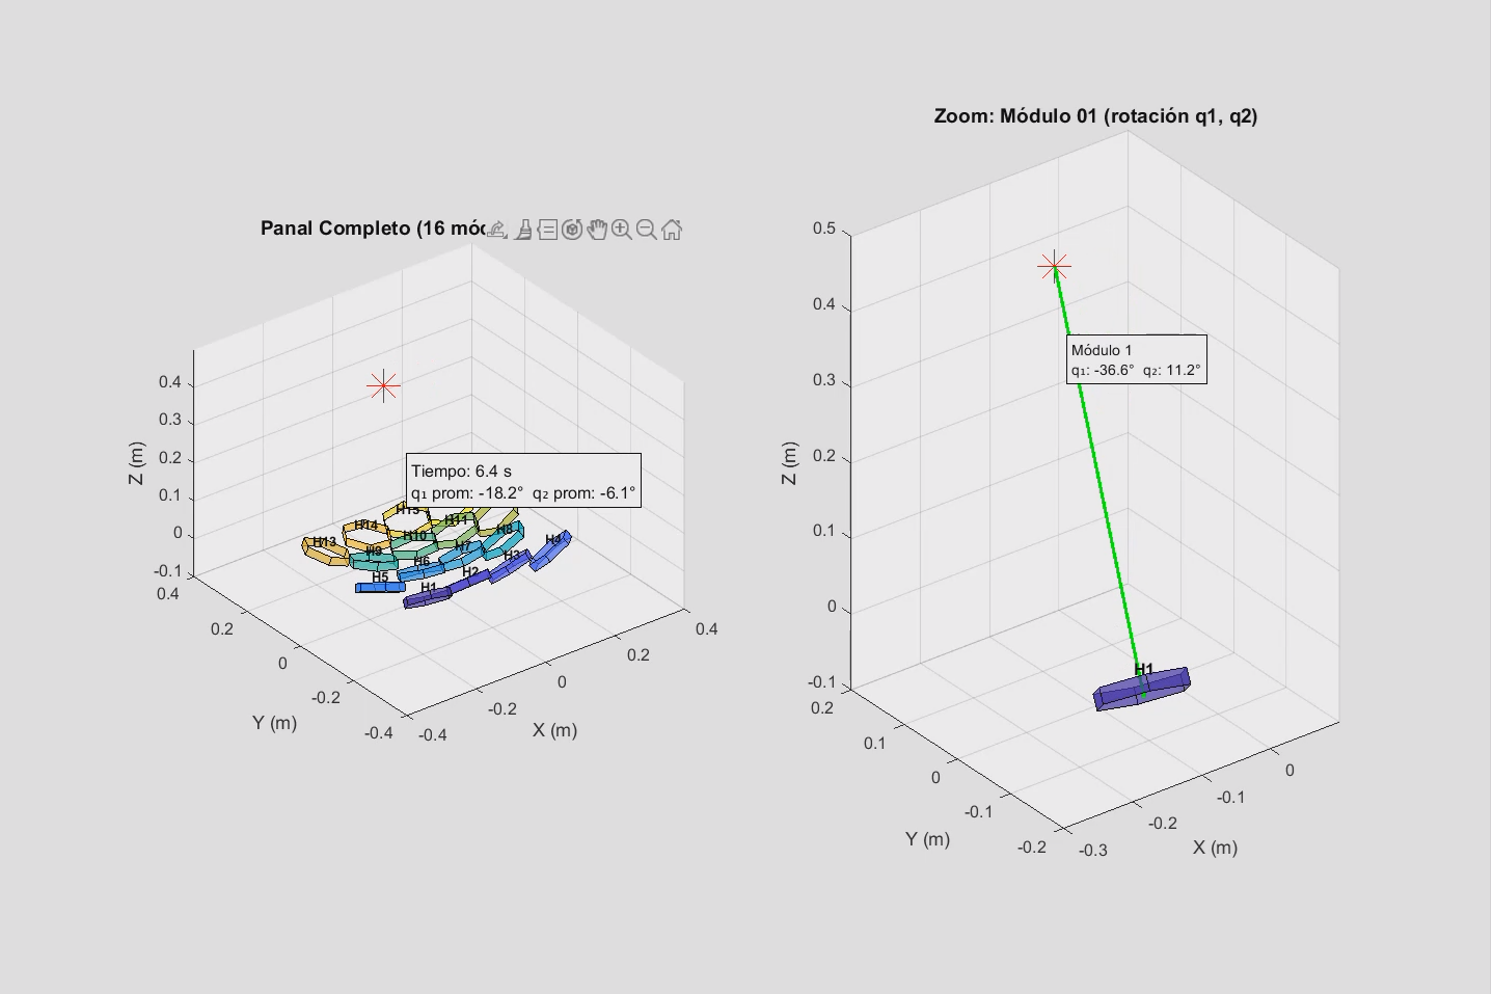
\includegraphics[width=0.47\linewidth]{s1}\label{fig:sim-a}}
\hfill
\subfloat[$t\approx10$ s.]{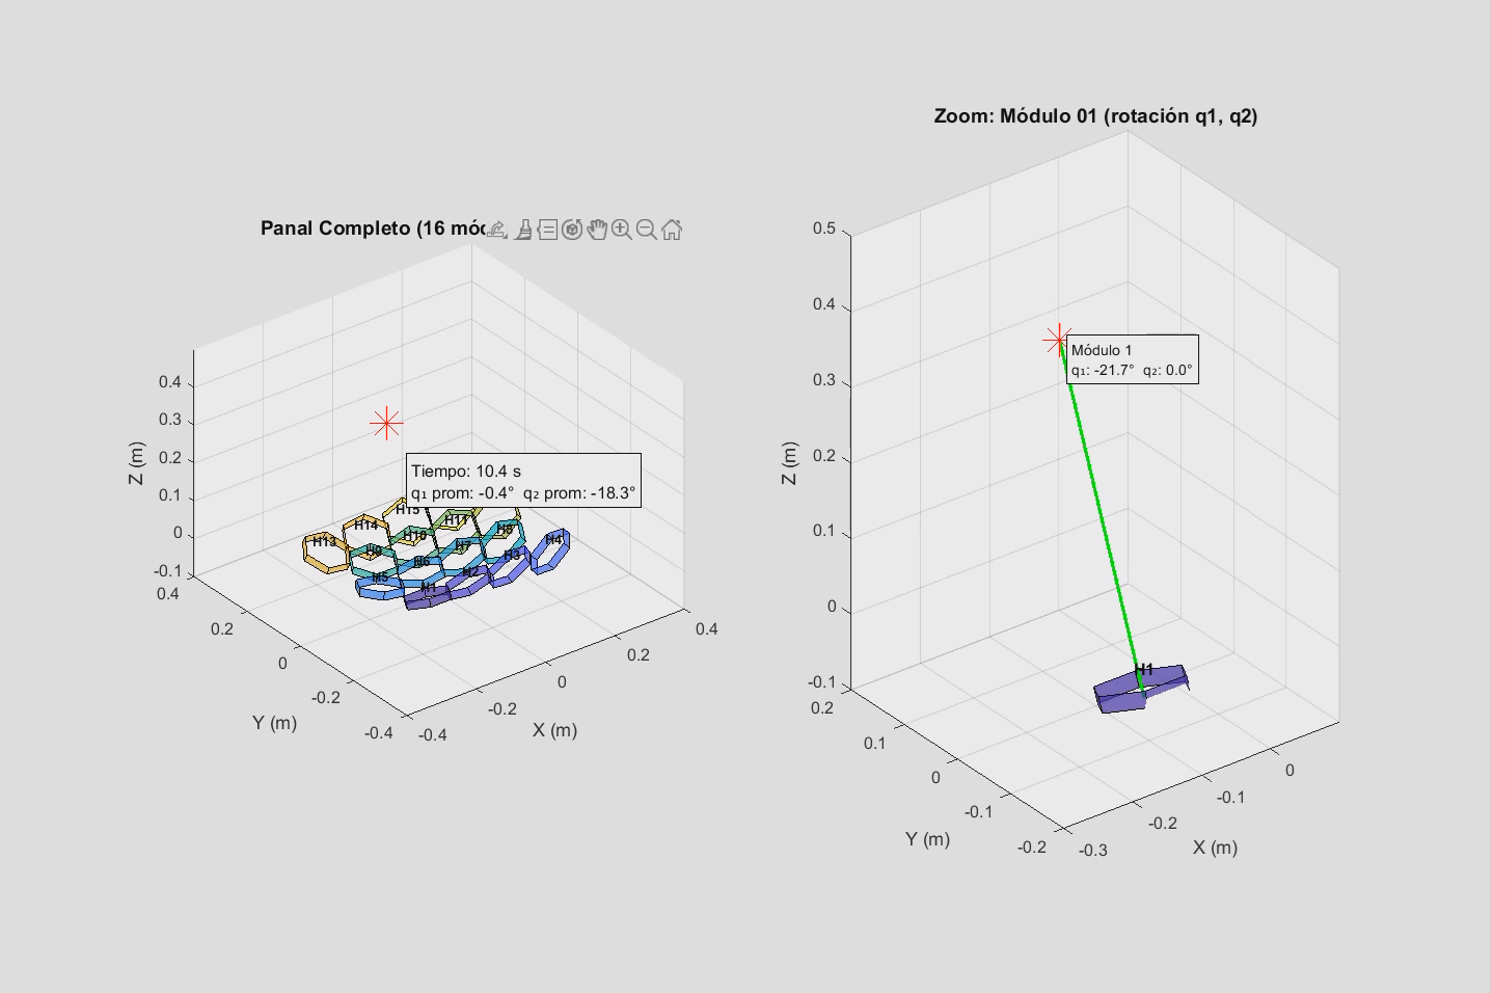
\includegraphics[width=0.47\linewidth]{s2}\label{fig:sim-b}}\\
\subfloat[$t\approx15$ s.]{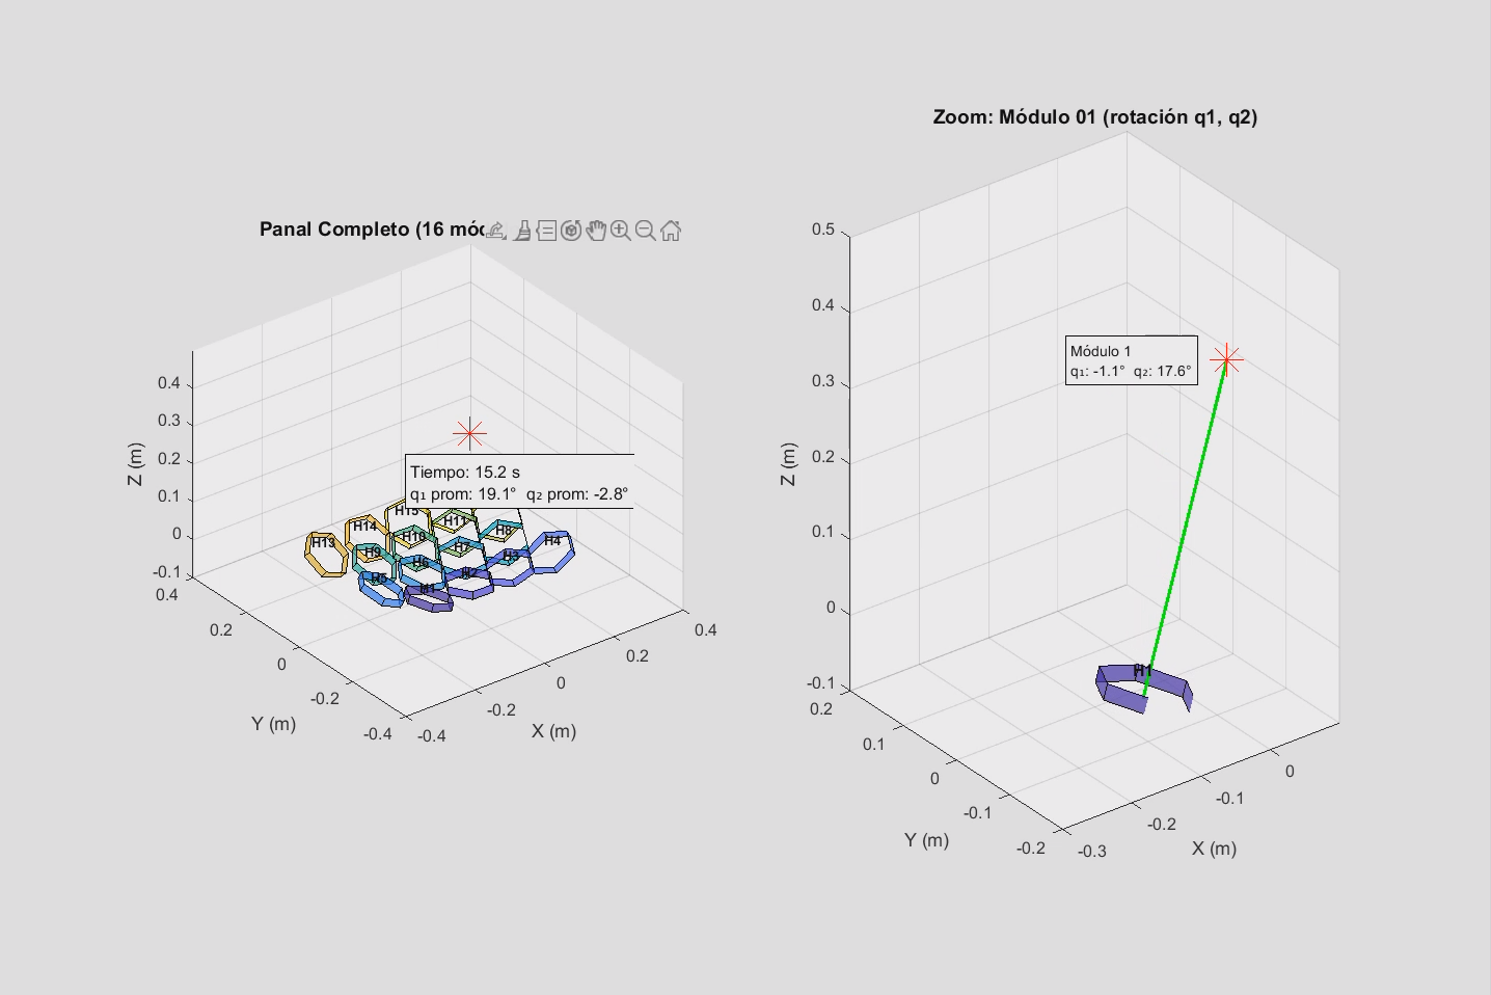
\includegraphics[width=0.47\linewidth]{s3}\label{fig:sim-c}}
\hfill
\subfloat[$t\approx18$ s.]{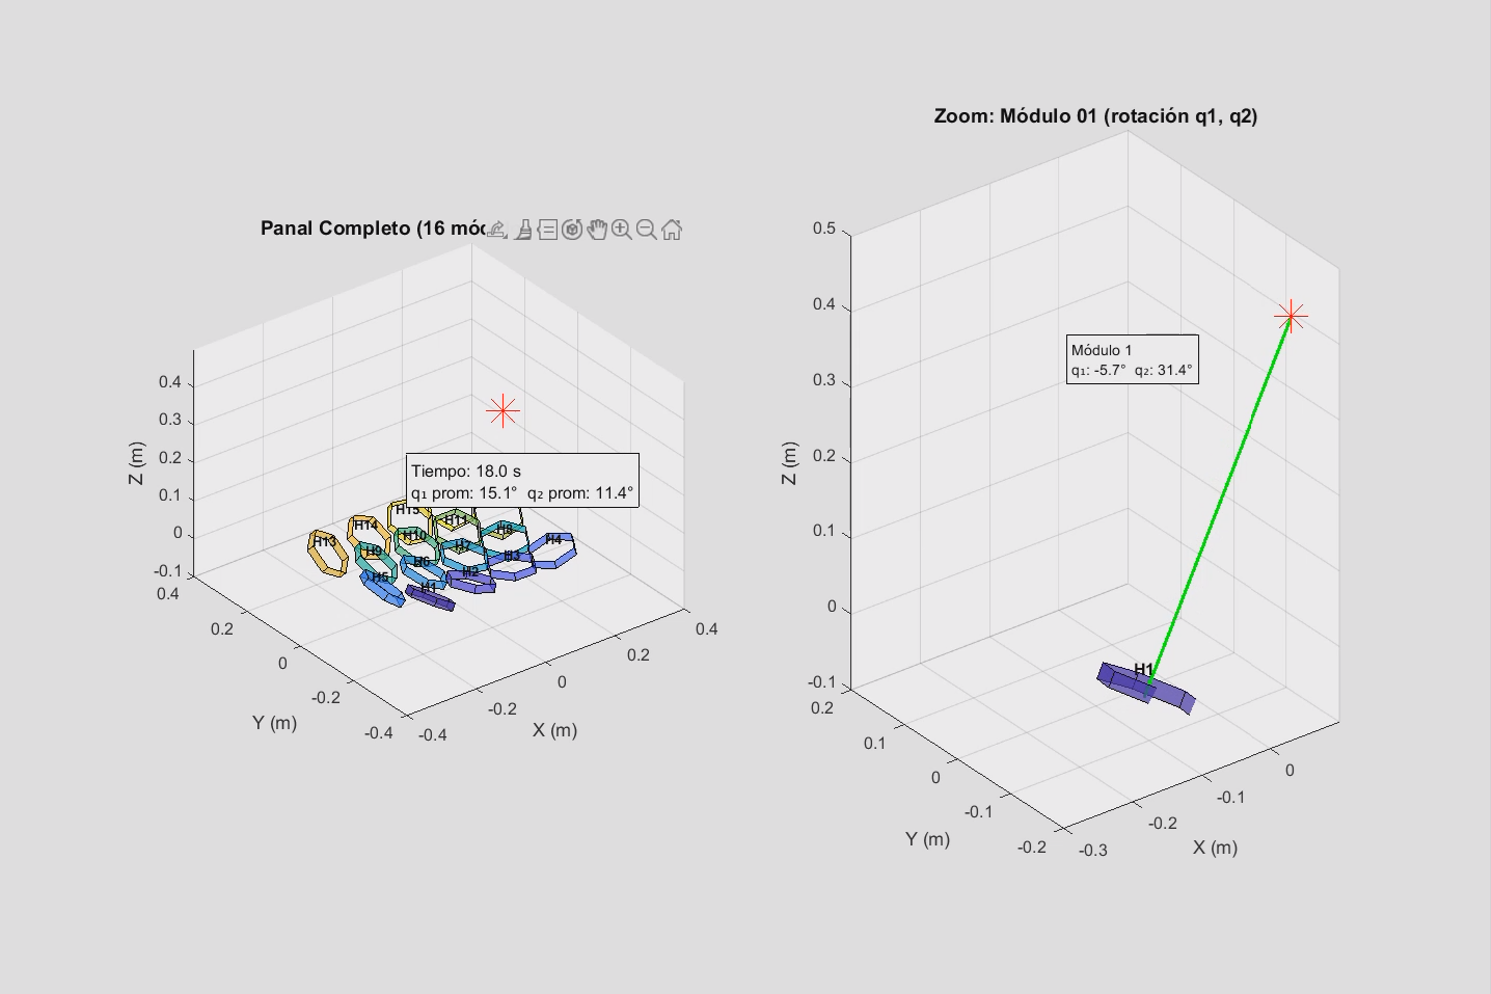
\includegraphics[width=0.47\linewidth]{s4}\label{fig:sim-d}}
\caption{MATLAB microtest of the 16-unit array following the circular target. The final Corte 1 figure should be regenerated with the corrected rotation convention and verification metric before submission.}
\label{fig:sim-sequence}
\end{figure}

\subsection{Preliminary Integration Risks and Mitigation}
\label{sec:risks}

Table~\ref{tab:risks} records risks already implied by the project requirements and kinematic model. The intent is to make each risk observable and testable during later integration rather than to treat it as an undocumented implementation detail.

\begin{table}[H]
\centering
\caption{Preliminary technical risk register for the sOFIa interaction loop.}
\label{tab:risks}
\scriptsize
\setlength{\tabcolsep}{2.5pt}
\begin{tabularx}{\columnwidth}{p{1.8cm}p{2.7cm}X}
\hline
\textbf{Risk} & \textbf{Technical effect} & \textbf{Planned mitigation / evidence} \\
\hline
Noisy hand landmarks or rapid classification changes & False gesture triggers and unstable mechanical reactions. & Per-hand landmark smoothing, temporal gesture rules, and output slew limiting; compare false activations before/after stabilization. \\
Camera unavailable & Perception loop cannot provide a valid command source. & Exception state in the GUI; stop/hold reaction and allow controlled recovery. \\
ESP32 disconnection or wireless loss & Command delivery is uncertain or stale. & Message acknowledgments, timeout/error codes, and automatic reconnection in the PC/ESP32 protocol. \\
Joint command outside physical range & Servo saturation and mismatch between desired and achieved pointing direction. & Explicit $\pm45^{\circ}$ clipping and angular-error measurement using Eq.~(\ref{eq:angular-error}). \\
Inverse-kinematics singularity & $q_1$ becomes undetermined when the target direction aligns with the local $x$ axis. & Detect $u_y\approx u_z\approx0$ and retain the previous valid $q_1$ command. \\
Multi-user ambiguity & A valid hand gesture may be associated with the wrong person or command context. & Associate detected hands with body poses before applying user-specific gesture context; include multi-user scenes in validation. \\
\hline
\end{tabularx}
\end{table}

\FloatBarrier

%=================================================================
% The following sections are intentionally omitted from the rendered
% Corte 1 draft. They belong to later cuts according to the checklist:
% Design and Implementation + Results (Corte 2), Discussion + Conclusions (Corte 3).
%=================================================================

\section*{Author Contributions}
Individual contribution statements are pending reconciliation with the team's GitHub/bitacora record and must be completed by the authors before submission.

\section*{Data Availability}
The source code, simulation files, figures, and LaTeX manuscript are maintained in the team's version-controlled project repository. A persistent repository link should be inserted in the final submission.

\section*{Acknowledgment}
The authors acknowledge the Laboratorio de Desarrollo de Soluciones Tecnol\'ogicas (LabDST) at ITESO for the sOFIa reference platform and technical project material. 

The authors also acknowledge the use of generative artificial intelligence tools to assist with the organization and structuring of the manuscript, as well as as a supplementary tool during the research process. All technical decisions, analyses, implementations, verification of information, and final content remain the responsibility of the authors.

\section*{Conflicts of Interest}
Conflict-of-interest status must be confirmed by all authors before final submission.

\balance
\bibliographystyle{IEEEtran}
\bibliography{bibliography}

\end{document}
